CSV-Files werden dazu verwendet, eine große Menge von Daten in einem File abzuspeichern. Diese Daten werden mithilfe von Semikolons, Beistrichen oder anderen Trennzeichen geteilt, siehe Abb. \ref{fig:impl:csvDateiEditor}. Durch diese Trennzeichen kann eine CSV-Datei jederzeit übersichtlich in Excel geöffnet werden. Mithilfe von CSV-Files können Daten ohne Probleme von einer Anwendung zu einer anderen Anwendung transferiert werden. \cite{csvOrJson}

\begin{figure}[h t]
    \centering
    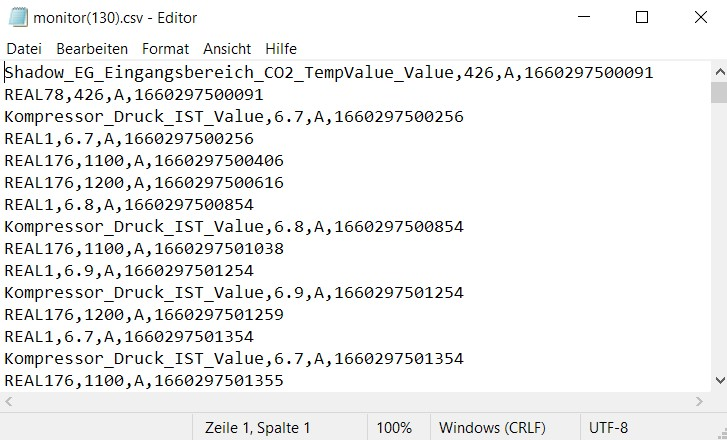
\includegraphics[scale=0.5]{pics/csvFileEditor.jpg}
    \caption{Beispiel einer CSV-Datei}
    \label{fig:impl:csvDateiEditor}
  \end{figure}
  